\section{\textit{Betweenness Centrality}}

O algoritmo de \textit{Betweeness Centrality}(BC) é utilizado para o 
estudo de redes sociais devido a indicar a medida de centralidade para cada 
vértice da rede a que foi aplicado, isto é, calcula para cada vértice um grau de 
importância/influência. 

Para calcular a centralidade de cada vértice é necessário calcular os 
caminhos mais curtos entre todos os vértices. A fórmula para calcular a 
\textit{Betweeness Centrality} para um dado vértice v é dada pela fórmula 
\ref{eq:bc}.

\begin{equation}
	Bc(v) = \sum\limits_{s \neq v \neq t} 
\frac{\sigma_{st}(v)}{\sigma_{st}}
	\label{eq:bc}
\end{equation}
$\sigma_{st}-$~caminhos mais curtos do vértice s para o vértice t.\\
$\sigma_{st}(v)-$ $\sigma_{st}$ dos quais passam em v.\\

É possível normalizar a  fórmula \ref{eq:bc} conseguindo-se uma BC normalizada usando a fórmula 
\ref{eq:normalizedbc}

\begin{equation}
	N(Bc(v)) = \frac{Bc(v) - min(BC)}{max(BC)-min(BC)} 
	\label{eq:normalizedbc}
\end{equation}
$max(BC)-$ a maior BC calculada.\\
$min(BC)-$ a menor BC calculada.\\

Para calcular a \textit{Betweenness Centrality} pode-se usar um algoritmo de 
\textit{Breath First Search} (BFS) modificado de modo a calcular os caminhos 
mais curtos entre todos os vértices. 

\paragraph{Exemplo}
A \textit{Betweenness Centrality} para o vértice B no grafo representado pela 
figura \ref{fig:bcexample} pode ser calculada do seguinte modo:

\begin{math}
BC(b) = \sigma_{ac}(B)/\sigma_{ac} + \sigma_{ad}(B)/\sigma_{ad} + 
\sigma_{cd}(B)/\sigma_{cd} = 1/1 + 1/1 + 1/1 = 3
\end{math}

\begin{math}
N(Bc(v)) =  (Bc(B) - min(BC))/(max(BC) - min(BC)) = (3 - 0) / ( 3 - 0 )=1  
\end{math}


\begin{figure}
\center
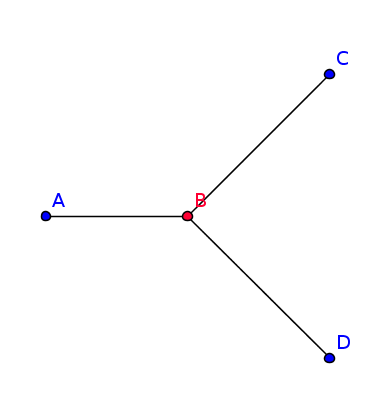
\includegraphics[scale=0.5]{bcexample}
\caption{Grafo de exemplo para calcular a BC.}\label{fig:bcexample}
\end{figure}
\subsection{Algoritmo distribuído para calcular a Betweenness Centrality}
O algoritmo distribuído consiste em calcular os caminhos mais curtos dentre todos os vértices inicialmente de forma distribuído, sendo similar à implementação do 
\textit{Shortest Path} distribuído. Após se obter todos os caminhos mais curtos 
então pode-se proceder ao cálculo da \textit{Betweeness Centrality}. Como o algoritmo tem elevados custos de memória esta versão apenas fará os caminhos mais curtos de começando em alguns vértices escolhidos previamente, nomeados de vértices iniciais. A \textit{Betweeness Centrality} é calculada para todos os vértices mas as mensagens iniciais vêm apenas dos vértices iniciais.
 
Para o algoritmo distribuído é necessário a existência de dois tipos de 
mensagens. Um dos tipos de mensagem necessita de informação suficiente para a realização de uma \textit{Breath First Search}(\textbf{mensagem de progresso}), sendo esta 
informação composta pelo identificador do vértice inicial, o vértice que enviou a mensagem e a distância 
até ao momento. Tem também de existir 
uma mensagem que indica que os vértices fazem parte de um caminho mais curto. 

Cada vértice terá como informação, para cada vértice inicial, os adjacentes em que o caminho passa para chegar a si (predecessores) e também a 
lista de mensagens de caminhos mais curtos recebidas para cada vértice inicial, com elementos compostos pelo \verb|id| do vértice inicial e o \verb|id| do do vértice que enviou a mensagem. O algoritmo distribuído em que se pode tanto normalizar ou não os 
valores para cada vértice pode ser descrito segundo o algoritmo~\ref{alg:distbc}.

\begin{algorithm}
  \caption{Algoritmo distribuído para calcular a BC.}
  \label{alg:distbc}
  \begin{enumerate}  
    \item No primeiro \textit{superstep}, começa-se por enviar 
  para os vértices adjacentes a mensagem de começo com distância 0.
    \item Caso se queira normalizar, verificar o estado global (previamente 
agregado) para se saber se nenhum vértice enviou mensagens. Caso nenhum vértice 
tenha enviado mensagens então procede-se ao passo da normalização descrito no 
algoritmo \ref{alg:normbc}.
    \item Iterar sobre as mensagens recebidas.
    \begin{enumerate}
      \item Caso seja uma mensagem de progresso então são processadas segundo o 
algoritmo \ref{alg:msgprogbc}.
      \item Caso sejam mensagens a indicar um caminho curto então são 
processadas de acordo com o algoritmo \ref{alg:msgpathbc}
    \end{enumerate}
      \item Após serem processadas todas as mensagens, calcular o valor da 
BC para o vértice seguindo a fórmula \ref{eq:bc} para os novos caminhos mais 
curtos e somar ao valor atual da BC do vértice.
      \item Caso não se queira normalizar pode-se sempre, no final de cada 
\textit{superstep} fazer \textit{halt} ao vértice. Caso contrário, os vértices 
têm de se manter acordados e é agregado de forma global, em todos os 
\textit{supersteps}, se o vértice enviou ou não mensagens.
  \end{enumerate}
\end{algorithm}

\begin{algorithm}
  \caption{Algoritmo distribuído para calcular a BC. Processamento das 
mensagens de progresso recebidas.}
  \label{alg:msgprogbc}
  \begin{enumerate}
		\item Todas as mensagens com o mesmo vértice inicial e a mesma distância são consideradas o caminho mais curto se o vértice atual não tiver recebido uma mensagem deste vértice inicial anteriormente.
    \item Caso seja um caminho mais curto então adicionar à lista de 
predecessores do vértice inicial o vértice que enviou a mensagem (se o 
vértice inicial for diferente do vértice que enviou a mensagem). Deve-se 
ter em conta que no mesmo \textit{superstep} pode-se receber mais do que uma 
mensagem proveniente do mesmo vértice inicial.
    \item As mensagens que originaram caminhos mais curtos são enviadas a todos os adjacentes que não são predecessores para este vértice inicial,  atualizando a informação vértice que enviou a mensagem para o vértice atual e incrementando a distância.
    \item Para todos os caminhos mais curtos encontrados e para os 
seus respetivos predecessores, enviar uma mensagem de caminho mais curto em que o vértice de destino é o vértice atual e o vértice inicial é o vértice inicial do caminho.
  \end{enumerate}
\end{algorithm}

\begin{algorithm}
  \caption{Algoritmo distribuído para calcular a BC. Processamento das 
mensagens recebidas a indicar um caminho mais curto.}
  \label{alg:msgpathbc}
  \begin{enumerate}  
     \item Processar todas as mensagens de modo a contar o número de 
caminhos que passam no vértice com o mesmo par \{vértice inicial, vértice destino\}. 
Para cada par, guardar informação de número caminhos que existem desde o 
vértice inicial até ao de vértice destino.
     \item Replicar as mensagens para os predecessores que não forem o vértice inicial que originou o caminho.
  \end{enumerate}
\end{algorithm}

\begin{algorithm}
  \caption{Algoritmo distribuído para calcular a BC. Passo de normalização.}
  \label{alg:normbc}
  \begin{enumerate} 
    \item Antes do \textit{superstep} em que se normaliza:
    \begin{enumerate}  
      \item Agregar o valor mínimo da BC num agregador global para o 
efeito, isto é, este agregador tem de estar preparado para ficar apenas com o 
valor mínimo dos que lhe foram entregues.
      \item Agregar o valor máximo da BC num agregador global, estando este 
também de ter sido concebido para ficar apenas com o valor máximo de todos os 
valores.
    \end{enumerate}
    \item No \textit{superstep} a seguir à agregação pode-se então para 
cada vértice calcular o valor normalizado segundo a fórmula 
\ref{eq:normalizedbc}.
  \end{enumerate}
\end{algorithm}


\clearpage
